\documentclass[preprint,10pt]{sigplanconf}

\usepackage{amsmath}

\usepackage{xspace}
\usepackage[caption=false]{subfig}

\usepackage{listings}

%% To import in the preambule
%\usepackage{listings}

% "define" Scala
\lstdefinelanguage{scala}{
  alsoletter={@,=,>},
  morekeywords={abstract, case, catch, class, def, do, else, extends, false, final, finally, for, foreach, if, implicit, import, match, new, null, object, 
override, package, private, protected, requires, return, sealed, super, this, throw, trait, try, true, type, val, var, while, with, yield, domain, 
postcondition, precondition,invariant, constraint, assert, forAll, in, _, async, asyncAt, finish, at},
  sensitive=true,
  morecomment=[l]{//},
  morecomment=[s]{/*}{*/},
  morestring=[b]"
}

\newcommand{\codestyle}{\small\sffamily}

\newcommand{\SAND}{\mbox{\tt \&\&}\xspace}
\newcommand{\SOR}{\mbox{\tt ||}\xspace}
\newcommand{\MOD}{\mbox{\tt \%}\xspace}
\newcommand{\DIV}{\mbox{\tt /}\xspace}
\newcommand{\PP}{\mbox{\tt ++}\xspace}
\newcommand{\PL}{\mbox{\tt +}\xspace}
\newcommand{\MM}{\mbox{\tt {-}{-}}\xspace}
\newcommand{\RA}{\Rightarrow}
\newcommand{\EQ}{\mbox{\tt ==}}
\newcommand{\NEQ}{\mbox{\tt !=}}
\newcommand{\SLE}{\ensuremath{\leq}}
\newcommand{\SGE}{\ensuremath{\geq}}
\newcommand{\SGT}{\mbox{\tt >}}
\newcommand{\SLT}{\mbox{\tt <}}
\newcommand{\rA}{\rightarrow}
\newcommand{\lA}{\leftarrow}

% Default settings for code listings
\lstset{
  language=scala,
  showstringspaces=false,
  columns=fullflexible,
  mathescape=true,
  numbers=none,
  numberstyle=\tiny,
  basicstyle=\codestyle
} 



\usepackage{defs}

\begin{document}

\special{papersize=8.5in,11in}
\setlength{\pdfpageheight}{\paperheight}
\setlength{\pdfpagewidth}{\paperwidth}

\conferenceinfo{CONF 'yy}{Month d--d, 20yy, City, ST, Country} 
\copyrightyear{20yy} 
\copyrightdata{978-1-nnnn-nnnn-n/yy/mm} 
\doi{nnnnnnn.nnnnnnn}

% Uncomment one of the following two, if you are not going for the 
% traditional copyright transfer agreement.

%\exclusivelicense                % ACM gets exclusive license to publish, 
                                  % you retain copyright

\permissiontopublish             % ACM gets nonexclusive license to publish
                                  % (paid open-access papers, 
                                  % short abstracts)

% \titlebanner{banner above paper title}        % These are ignored unless
% \preprintfooter{short description of paper}   % 'preprint' option specified.

\title{Distributed Programming in Scala with APGAS}

\authorinfo{Name1 \and Name2\and Name3}
           {IBM T.J. Watson Research Center}
           {\{name1,name2,name3\}@us.ibm.com}

\maketitle

\begin{abstract}
\apgas (Asynchronous Partitioned Global Address Space) is a model for
concurrent and distributed programming, known primarily as the foundation of
the X10 programming language. In this paper, we present an implementation of
this model as an embedded domain-specific language for Scala. We illustrate
common usage patterns and contrast with alternative approaches available to
Scala programmers. In particular, through two full-fledged examples, we
illustrate how \apgas-style programs compare to idiomatic Akka implementations.
We demonstrate the use of active messages, SPMD, distributed termination, and
fault-tolerance.

\end{abstract}

% \category{CR-number}{subcategory}{third-level}

% general terms are not compulsory anymore, 
% you may leave them out
% \terms
% term1, term2
% 
% \keywords
% keyword1, keyword2

\section{Introduction}

The APGAS programming model~\cite{amp10}---Asynchronous Partitioned Global Address Space---is simple but powerful
model of concurrency and distribution. It combines PGAS with asynchrony.
In (A)PGAS the computation and data in an application are logically partitioned into places.
In APGAS the computation is further organized into lightweight asynchronous tasks.
With these, APGAS can express both
regular and irregular parallelism, message-passing-style and
active-message-style computations, fork-join and bulk-synchronous
parallelism.  In contrast to hybrid models like MPI+OpenMP, the same
constructs underpin both intra- and inter-place concurrency.

The X10 programming language~\cite{oopsla05} augments a familiar imperative, strongly-typed, garbage-collected, object-oriented language with the APGAS model. X10 is implemented with two backends. On the managed backend, X10
compiles into Java and runs on a cluster of JVMs. On the native backend, X10 compiles into C++ and generates a native binary
for execution on scale-out systems.
X10, and by extension
\apgas, has been used successfully to implement distributed applications
running across tens of thousands of cores~\cite{TardieuETAL14X10ApgasAtPetascale}.
The recently developed APGAS library for Java \cite{APGASJava} provides an alternative to X10 for programmers interested in the \apgas model but not willing to buy into a new programming language or development platform, which may not be possible for an array
of reasons.

To expose more programmer to APGAS, we propose to realize APGAS an as embedded domain-specific language for Scala. 
Scala welcomes library-based extensions and has been a pioneer on
the JVM for alternative concurrency paradigms. Notably, the original actor
library and its more recent successor Akka are examples of both. 
X10 shares ancestry and inspiration with Scala, and the
facilities in Scala for library-defined language extensions make the code look
almost exactly like X10 programs.

Section~\ref{sec:apgas} describes the APGAS programming model and its embedding in Scala. We demonstrate two examples programs: \kmeans in Section~\ref{sec:kmeans} and Unbalanced Tree Search in Section~\ref{sec:uts}. Section~\ref{sec:serialization} discusses implementation and Section~\ref{sec:conclusion} concludes the paper.

We hope that people will embrace \apgas, either as a substitute for or as a
complement to other concurrency libraries. Examples throughout the paper are
verbatim Scala \apgas code. 


\section{Overview of \apgas in Scala}
\label{sec:apgas}.

A {\em place} is an abstraction of mutable, shared-memory region and worker threads operating on this memory.
A single application typically runs over a collection of places. In this work, each place is implemented as a separate JVM.

A {\em task} is an abstraction of a sequence of computations. In this work, a task is specified as a block.
Each task is bound to a particular place. 
A task can spawn local and remote tasks, i.e., tasks to be executed in the same place or elsewhere.

A local task shares the heap of the parent task. A remote task executes on a snapshot of the parent task's heap captured when the task is spawned. A task can instantiate \emph{global references} to objects in its heap to work around the capture semantics.
Global references are copied as part of the snapshot but not the target objects. A global reference can only be dereferenced
at the place of the target object where it resolves to the original object.

A task can wait for the termination of all the tasks transitively spawned from it.
Thanks to global references, remote tasks, and termination control,
a task can indirectly manipulate remote objects.

The two fundamental control structures in APGAS are
 \lstinline{asyncAt}, and \lstinline{finish}, whose signatures in
the Scala implementation are:
\begin{lstlisting}
  def asyncAt(place: Place)(body: $\RA$Unit) : Unit
  def finish(body : $\RA$Unit) : Unit
\end{lstlisting}
As is common in Scala libraries, we use by-name arguments to capture blocks.

The \lstinline{async} construct spawns an asynchronous task at place \lstinline{p} and returns
immediately. It is therefore the primitive construct for both \emph{concurrency} and \emph{distribution}.
The \lstinline{finish} construct detects termination: an invocation of
\lstinline{finish} will execute its body and block until all nested invocations
of \lstinline{asyncAt} have completed. The set of \lstinline{asyncAt} invocations
that are controlled includes all recursive invocations, including all remote
ones. This makes \lstinline{finish} a powerful contribution of \apgas.

Because spawning local tasks is so common, we have an optimized version of \lstinline{asyncAt} for this purpose with signature:
\begin{lstlisting}
  def async(body: $\RA$Unit) : Unit
\end{lstlisting}  

TODO

\begin{lstlisting}
  def at[T:Serialization](place: Place)(body: $\RA$T) : T
\end{lstlisting}
We discuss the \lstinline{Serialization} type class in
Section~\ref{sec:serialization}.


The primitive construct for \emph{distribution} is \lstinline{at}. The invocation
\begin{lstlisting}
  val r = at(p) { work() }
\end{lstlisting}
executes the method \lstinline{work} at place \lstinline{p}, and blocks until
it terminates and returns the result. Asynchronously spawning tasks at remote places can be achieved by composing the two constructs:
\begin{lstlisting}
  at(p) { async { work() }}
\end{lstlisting}
This operation is so common that we have an semantically equivalent but optimized version with the signature
\begin{lstlisting}
  def asyncAt(place: Place)(body: $\RA$Unit) : Unit
\end{lstlisting}

Finally, \lstinline{finish} detects termination: an invocation of
\lstinline{finish} will execute its body and block until all nested invocations
of \lstinline{async} have completed. The set of \lstinline{async} invocations
that are controlled includes all recursive invocations, including all remote
ones. This makes \lstinline{finish} a powerful contribution of \apgas.

Fibonacci

SPDM

Memory: PlaceLocal, PlaceLocalRef

Place failure.

\subsection{Similarities and Differences with Futures and Actors}

Discuss future vs.\ async (returning void means no value). Future can be awaited anywhere, but must be awaited ``manually''.

finish counts (including distributed tasks!) and has no real equivalent.

Actors: unified model for concurrency and distribution.

Handling failures: Try vs Exception vs. Messages

Async at: active messages: get executed "immediately", actor messages handled one-by-one.

In the following sections, we highlight some of the points above through two
benchmarks, \kmeans clustering and unbalanced tree search.


% \newsavebox\patternRemoteEval
\begin{lrbox}{\patternRemoteEval}
\begin{lstlisting}
v = at(p) {
  evalThere(arg1, arg2)
}
\end{lstlisting}
\end{lrbox}

\newsavebox\patternActiveMessage
\begin{lrbox}{\patternActiveMessage}
\begin{lstlisting}
asyncAt(p) {
  runThere(arg1, arg2)
}
\end{lstlisting}
\end{lrbox}

\newsavebox\patternRecursiveParallelDecomposition
\begin{lrbox}{\patternRecursiveParallelDecomposition}
\begin{lstlisting}
def fib(n : Long) : Long = {
  if(n < 2) n else {
    var f1, f2 = 0L
    finish {
      async { f1 = fib(n - 1) }
      f2 = fib(n - 2)
    }
    f1 + f2
  }
}
\end{lstlisting}
\end{lrbox}

\newsavebox\patternSPMD
\begin{lrbox}{\patternSPMD}
\begin{lstlisting}
finish {
  for(p $\lA$ places) {
    at(p) {
      async { runEverywhere(arg1, arg2) }
    }
  }
}
\end{lstlisting}
\end{lrbox}

\begin{figure*}
\centering
\subfloat{\usebox\patternRemoteEval}\qquad
\subfloat{\usebox\patternActiveMessage}\qquad
\subfloat{\usebox\patternRecursiveParallelDecomposition}\qquad
\subfloat{\usebox\patternSPMD}\qquad
\caption{Common \apgas patterns in Scala.\label{fig:apgas-patterns}}
\end{figure*}

% Figure~\ref{fig:apgas-patterns} shows patterns.

\section{Distributed \kmeans Clustering}
\label{sec:kmeans}

The \kmeans benchmark uses Lloyd's algorithm~\cite{Lloyd1982Least} to divide a
set of points in a $d$-dimensional space into $k$ disjoint clusters.  Given an
arbitrary set of initial clusters, the algorithm iterates over the following
steps:
\begin{enumerate}
  \item For each point, assign that point to whichever cluster is closest (by
Euclidean distance to the cluster centroid).
  \item For each cluster, update the centroid (the arithmetic mean of all
points assigned to that cluster).
\end{enumerate}
Distributed computation is straightforward: each process holds a portion of the
points and computes cluster assignments and centroid contributions for each
point. At each iteration, a master process collects all centroid contributions,
computes the aggregates, checks if the computation has converged, and if not,
communicates the updated values to all workers.

Figure~\ref{fig:kmeansapgas} shows the main structure of a distributed \kmeans
computation with \apgas. The state is split between the master's view of 1) the
centroids and 2) the contributions being collected, and the workers'
place-local memory, comprising a subset of points and the local view of the
centroids. The place-local memory is held in \lstinline{local}, of type
\lstinline{GlobalRef[LocalData]}.

The structure of the computation, including the distribution
aspect, is fully explicit in the code: the outermost \lstinline{while} loop
iterates until convergence, the \lstinline{for} loop spawns an activity to be run asynchronously at each place as indicated by \lstinline{asyncAt}, which in turn spawns a remote activity at the master place to combine the place's local view with the master's view.
Finally, \lstinline{finish} ensures that all remote work has completed before
proceeding to the next iteration.
\begin{figure}
\begin{lstlisting}
class ClusterState extends Serializable {
  val centroids $\EQ$ Array.ofDim[Float](K, D)
  val counts $\EQ$ Array.ofDim[Int](K)
}
class LocalData(val points: ..., val state: ClusterState) { ... }
val local: LocalData $\EQ$ GlobalRef.forPlaces(places) { ... }
val masterState $\EQ$ new ClusterState()
val masterRef $\EQ$ SharedRef.make(masterState)
val currentCentroids $\EQ$ Array.ofDim[Float](K, D)
while (!converged()) {
  finish {
    reset(newCentroids); reset(newCounts)
    for (p $\lA$ places) {
      asyncAt(place) {
        val pState = local().state
        val points = local().points
        compute(currentCentroids, points, pState)
        asyncAt(masterRef.home) {
          val masterCentroids $\EQ$ masterRef().centroids
          masterCentroids.synchronized {
            ... /* add elements from pState.centroids */ }
          val masterCounts $\EQ$ masterRef().counts
          masterCounts.synchronized {
            ... /* add elements from pState.counts */ }
        }
      }
  } } }
  ... // normalize centroids by counts
  copyArray(masterState.centroids, currentCentroids)
}
\end{lstlisting}
\caption{Code structure for \kmeans in \apgas.\label{fig:kmeansapgas}}
\end{figure}
An aspect of the code that can be harder to grasp is the movement of data: the
value of \lstinline{currentCentroids} is sent from the master to a worker by letting the variable be captured in the closure passed to \lstinline{asyncAt}.
Note that while \lstinline{local} is a
\lstinline{GlobalRef} and is therefore never serialized implicitly, we use
\lstinline{apply} to dereference it and thus pass a copy of the data of type
\lstinline{LocalData} to the master process in the nested \lstinline{asyncAt}.
Finally, note that the code that adds the contribution of a worker to the master values is synchronized to avoid data races.

For contrast, Figure~\ref{fig:kmeansakka} shows the related parts of an
actor-based implementation of \kmeans clustering using Akka.
\begin{figure}
\begin{lstlisting}
  class Master(...) extends Actor {
    val workers: Seq[ActorRef] $\EQ$ ...
    val centroids, newCentroids $\EQ$ Array.ofDim[Float](K, D)
    val newCounts $\EQ$ Array.ofDim[Int](K)
    var received $\EQ$ 0
    override def receive $\EQ$ {
      case Run $\RA$ if(!converged()) {
        reset(newCentroids); reset(newCounts)
        received $\EQ$ 0
        workers.foreach(_ ! Update(centroids)) }
      case Updated(workerCentroids, workerCounts) $\RA$
        ... /* add elements from pState.centroids */ }
        ... /* add elements from pState.counts */ }
        received $\PEQ$ 1
        if(received $\EQEQ$ numWorkers) {
          ... // normalize newCentroids by newCounts
          copyArray(newCentroids, centroids)
          self ! Run }
  } }
  class Worker(...) extends Actor {
    val points $\EQ$ ...
    val localCentroids $\EQ$ ...; val localCounts $\EQ$ ...
    override def receive $\EQ$ {
      case Update(centroids) $\RA$
        compute(centroids, this, ...)
        sender ! Updated(localCentroids, localCounts)
  } }
\end{lstlisting}
\caption{Code structure for \kmeans in Akka.\label{fig:kmeansakka}}
\end{figure}
Almost as a dual to the \apgas implementation, the movement of data is entirely
explicit, but the control flow must be inferred from the flow of messages: the
master actor sends itself \lstinline{Run} messages to continue the computation,
and must keep count of how many \lstinline{Updated} messages it received from
workers to know when an iteration is complete. There is no need for data
synchronization, as the model enforces that message processing within an actor
is always a sequential operation.

\section{Unbalanced Tree Search}
\label{sec:uts}

The Unbalanced Tree Search benchmark (UTS) measures the rate of traversal of a
tree generated on the fly using a splittable random number generator
\cite{lcpc06}. The problem specification describes several cryptographic laws
for computing the number of children of a node and their hashes. This results
in trees that are deterministic but unbalanced in unpredictable ways. 

A sequential implementation of UTS is straightforward: the code maintains a
work list of nodes to expand, and repeatedly pops one and adds its children to
the list. It terminates when the list is empty, and returns the number of
popped elements. In contrast, a parallel and distributed implementation of UTS
is a challenge because of imbalance. We implement distributed work stealing
with lifelines \cite{ppopp11}.

\paragraph{Distributed Algorithm.} A fixed collection of workers collaborate on
the traversal. The workers are organized in a ring. Each worker maintains a
work list of pending nodes to visit and count of nodes already traversed. Each
worker primarily processes its own list, following the sequential algorithm. If
the list becomes empty, the worker tries to steal nodes from another random
worker. If this fails because the victim's work list is empty as well, the
worker sends a request to the next worker in the ring---its lifeline---and
stops. If this lifeline now has or later obtains nodes to process, it deals a
fraction of these nodes to the requester. One work list is initialized with the
root node of the traversal. The traversal is complete when all workers have
stopped and there are no deal messages from a lifeline in flight. The sum of
the node counts is computed at that point.

\paragraph{State Machine.} Each worker can be in one of three states:
\begin{itemize}
\item \lstinline{work}: the worker is processing nodes from its work list;
\item \lstinline{wait}: the worker is attempting to steal nodes from a random victim and waiting for the result;
\item \lstinline{idle}: the worker has signaled its lifeline and stopped.
\end{itemize}
Figure~\ref{fig:uts-state} shows these states and the possible transitions as a
graph. The transitions---the edges---are annotated with the events associated
with them. E.g., the \lstinline{NoDeal}/\lstinline{LifelineReq} transition from
the wait state to the idle state denotes that this transition takes places upon
receiving the \lstinline{NoDeal} message and involves sending the \lstinline{LifelineReq}
message.
\begin{figure}
\centering
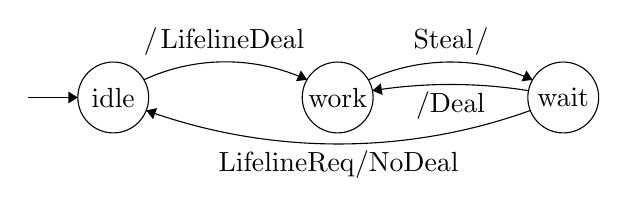
\begin{tikzpicture}[scale=0.15]
\tikzstyle{every node}+=[inner sep=0pt]
\draw [black] (16.5,-13.6) circle (3);
\draw (16.5,-13.6) node {\lstinline{idle}};
\draw [black] (35.5,-13.6) circle (3);
\draw (35.5,-13.6) node {\lstinline{work}};
\draw [black] (54.6,-13.6) circle (3);
\draw (54.6,-13.6) node {\lstinline{wait}};
\draw [black] (19.093,-12.1) arc (114.8182:65.1818:16.454);
\fill [black] (32.91,-12.1) -- (32.39,-11.31) -- (31.97,-12.22);
\draw (26,-10.08) node [above] {/\lstinline{LifelineDeal}};
\draw [black] (38.101,-12.113) arc (114.61614:65.38386:16.684);
\fill [black] (52,-12.11) -- (51.48,-11.32) -- (51.06,-12.23);
\draw (45.05,-10.1) node [above] {\lstinline{Steal}/};
\draw [black] (38.443,-13.022) arc (99.06897:80.93103:41.916);
\fill [black] (38.44,-13.02) -- (39.31,-13.39) -- (39.15,-12.4);
\draw (45.05,-13.1) node [below] {/\lstinline{Deal}};
\draw [black] (51.81,-14.703) arc (-70.22137:-109.77863:48.053);
\fill [black] (19.29,-14.7) -- (19.87,-15.44) -- (20.21,-14.5);
\draw (35.55,-18.04) node [below] {\lstinline{LifelineReq}/\lstinline{NoDeal}};
\draw [black] (9.3,-13.6) -- (13.5,-13.6);
\fill [black] (13.5,-13.6) -- (12.7,-13.1) -- (12.7,-14.1);
\end{tikzpicture}
\caption{State diagram for UTS workers.\label{fig:uts-state}}
\end{figure}
\paragraph{Implementation in \apgas.}

We illustrate below the handling of the \{ \lstinline{Steal}, \lstinline{Deal} \} pair of messages in the \apgas implementation.
\begin{lstlisting}
class Worker($\ldots$) extends PlaceLocal {
  val thieves: ConcurrentLinkedQueue[Place] = $\ldots$
  val workList: WorkList = $\ldots$
  $\ldots$
  def steal() : Unit = {
    val thief: Place = here
    val victim: Place = $\ldots$ // pick randomly
    synchronized { state = Wait(p) }
    uncountedAsyncAt(victim) {
      thieves.add(thief)
    }
    synchronized { while (state.isWait) { wait() } }
  }
  def distribute() : Unit = {
    $\ldots$ 
    while({ p = thieves.poll(); p != null}) {
      val wl = workList.split()

      uncountedAsyncAt(p) {
        synchronized {
          workList.merge(wl)
          state = Work
          notifyAll()
        }
      }
    }
  }
}
\end{lstlisting}

\paragraph{Distributed Termination.} Distributed termination detection is notoriously difficult to implement correctly and efficiently.
For instance in UTS, observing that all workers are idle does not guarantee that the traversal is complete as messages containing nodes to process might still be in flight. Thanks to \lstinline{finish}, an entire class of hard-to-reproduce data races is ruled out by construction in APGAS.
A combination of static and dynamic analyses can bring down the cost of termination detection~\cite{TardieuETAL14X10ApgasAtPetascale}. 

APGAS provides two state-of-the-art \lstinline{finish} implementations for fault-tolerant and non-fault-tolerant instantiations of the library. The core algorithm uses a distributed array of counters akin to the X10 implementation. Each place maintains the count of tasks that completed locally and separate counts for each place where it spawned tasks. These arrays of counters are pushed to the place of the task waiting on the \lstinline{finish}. Termination is signaled when all the sums of the per-place task counts are zero.


% TODO
% 
% Common implementation of WorkList. Show interface. Explain mutability and
% ownership are for performance.
% 
% Akka: implementation using vanilla actors (no akka-fsm). Work is split up by
% sending \lstinline{Work} messages to oneself. State transitions are implemented
% using \lstinline{become}.
% 
% Termination is difficult.
% 
% UTS: three problems, three solutions.
% 
% UTS \apgas: concurrency control implemented as multiple paradigms (synchronized
% data access, global invariants, active messages). Concurrency is more
% fine-grained.


% Scala performance

\paragraph{Performance.} We measured the rate of traversal of our Akka and
\apgas implementations of UTS in millions of nodes per second (Mn/s), using
32-way parallelism on a 48 core machine. We measured three configurations: 1)
\apgas implementation on 32 processes, 2) Akka implementation on 1 process with
32 worker actors, 3) Akka implementation on 32 processes, each with 1 worker
actor.\footnote{As places in \apgas are currently only realized as separate
processes, configuration 3) is closer in terms of communication constraints.}
We used \lstinline{akka-remote} for configuration 3), and the flexibility of
the actor model means that the distribution of workers per process is isolated
to a single invocation of \lstinline{.withDeploy}. The configurations achieved
269.4Mn/s, 286.8Mn/s, and 274.2Mn/s, respectively. This shows that the \apgas
code comes within 98\% and 93\% of the performance of the multi-process and
single-process Akka configurations, respectively.

%UTSAPGAS 32 places, 1 worker/place, depth 15
%[uts-apgas-32] depth: 15, performance: 4230646601/15.617225935 = 270.8961641848719M nodes/s
%[uts-apgas-32] depth: 15, performance: 4230646601/15.757630678 = 268.4824062355144M nodes/s
%[uts-apgas-32] depth: 15, performance: 4230646601/15.730685914 = 268.9422841527087M nodes/s

%UTSAkka 32 process, 1 actor/process, depth 15
%[actors-32] depth: 15, performance: 4230646601/15.605088175 = 271.1068693464784M nodes/s
%[actors-32] depth: 15, performance: 4230646601/15.478703563 = 273.3204744041263M nodes/s
%[actors-32] depth: 15, performance: 4230646601/15.208430648 = 278.1777225355172M nodes/s

%UTSAkka 1 process, 32 actors, depth 15
%[actors-32] depth: 15, performance: 4230646601/14.622429161 = 289.32584007886373M nodes/s
%[actors-32] depth: 15, performance: 4230646601/14.783925108 = 286.16531605065273M nodes/s
%[actors-32] depth: 15, performance: 4230646601/14.852197401 = 284.8498768751316M nodes/s


%UTSSequential depth 13
%[serial] depth: 13, performance: 264459392/27.782491057 = 9.518922959695061M nodes/s
%[serial] depth: 13, performance: 264459392/27.740853577 = 9.533210334207734M nodes/s
%[serial] depth: 13, performance: 264459392/27.538216937 = 9.603359309900553M nodes/s


% Java performance

%GlobalUTS 32 places, 1 worker/place, depth 15 (hacked non resilient)
%Depth: 15, Places: 32, Performance: 4230646601/15.191 = 278.48M nodes/s using 0 transactions
%Depth: 15, Places: 32, Performance: 4230646601/15.267 = 277.09M nodes/s using 0 transactions
%Depth: 15, Places: 32, Performance: 4230646601/15.138 = 279.46M nodes/s using 0 transactions

%MultiUTS 1 place, 32 workers, depth 15 (hacked non resilient)
%Depth: 15, Locations: 32, Performance: 4230646601/14.601 = 289.73M nodes/s using 0 transactions
%Depth: 15, Locations: 32, Performance: 4230646601/14.791 = 286.02M nodes/s using 0 transactions
%Depth: 15, Locations: 32, Performance: 4230646601/14.557 = 290.61M nodes/s using 0 transactions

%GlobalUTS 32 places, 1 worker/place, depth 15 (resilient map)
%Depth: 15, Places: 32, Performance: 4230646601/15.883 = 266.35M nodes/s using 1119 transactions


\section{Conclusion}
\label{sec:conclusion}

%\acks
%
%Acknowledgments, if needed.

% We recommend abbrvnat bibliography style.

\bibliographystyle{abbrvnat}

\bibliography{managed}

\end{document}
